\documentclass[TechnicalNoteMeteo.tex]{subfiles}

\begin{document}

The Monteregie Est region is located in southern Quebec, Canada, on the south shore of the St. Lawrence River. It covers a total area of 9032~km\textsuperscript{2}, from the St. Lawrence River at its northern limit to the border of the United States (states of New York and Vermont) at its southern limit (see Figure X).

This region has been the subject of an extensive characterization project within the ``Programme d'acquisition de connaissances sur les eaux souterraines du Québec'' (PACES) whose main objective was to prepare a realistic and concrete picture of the groundwater resources for the region \citep{carrier_portrait_2013}.

\subsection{Study Area}

The climate is characterized by significant seasonal differences in temperature, resulting in warm summers and cold winters. Precipitation, as rain or snow, are distributed rather evenly throughout the year.

Among all the weather stations for which data were available in and around the study area, a total of 32 was selected based on the availability and continuity of the weather data between 1980 and 2014. A list of these selected stations is presented in Table~X with their coordinates, altitude, total time periods for which data were available, mean annual cumulative precipitation, and mean annual air temperature. Most of these information are generated automatically by WHAT in the file ``weather\_datasets\_summary.log'' (see Section~\ref{subsec:folder_structure}).

\subsection{Materials and Method}


%\begin{table}[!ht]
%\newcommand{\nan}{\multicolumn{1}{c}{\textbf{nan}}}
%\newcolumntype{d}{D{.}{.}{3.1} } %decimal column as before
%\center
%\caption{List of selected weather stations in the study area and related information about missing data for the 1980-2014 period}
%\begin{tabular}{r>{\RaggedRight}p{2.8cm}*3{c}d*5{d}}
%\toprule
%\multicolumn{6}{c}{}&
%\multicolumn{5}{c}{Percentage of missing data (\%)} \\
%\cmidrule(r){7-11}
%\multicolumn{1}{c}{}&
%\multicolumn{1}{l}{Stations}  &
%\multicolumn{1}{c}{ID} &
%\multicolumn{1}{c}{Lat.} &
%\multicolumn{1}{c}{Lon.} &
%\multicolumn{1}{c}{Alt.}&
%\multicolumn{1}{c}{T\textsubscript{max}}&
%\multicolumn{1}{c}{T\textsubscript{min}}&
%\multicolumn{1}{c}{T\textsubscript{avg}}&
%\multicolumn{1}{c}{P\textsubscript{tot}}&
%\multicolumn{1}{c}{TOTAL}\\
%\midrule
% 1 & Auteuil & 7020392 & 45.65 & -73.73 & 53.0 & 20.8 & 19.1 & 22.8 & 18.4 & 20.3 \\
% 2 & Bonsecours & 7020828 & 45.40 & -72.27 & 297.2 & 4.7 & 5.1 & 6.3 & 3.2 & 4.8 \\
% \rowcolor{gray!30}
% 3 & Brome &  7020840 & 45.18 & -72.57 &  205.7 & 2.6 & 2.3 & 3.0 & 2.3 & 2.5 \\
% 4 & Bromptonville &  7020860 &  45.48 &  -71.95 &  130.0 & 3.9 & 4.2 & 6.0 & 1.8 & 4.0 \\ 
% 5 & Danville &  7021954 &  45.82 & -71.98 & 190.0 & 30.8 & 31.1 & 33.1& 30.2 & 31.3 \\
% \rowcolor{gray!30}
% 6 & Drummondville  & 7022160 & 45.88 & -72.48 & 82.3 & 2.5 & 2.4 & 3.4 & 1.8 & 2.5 \\
% 7 & Farnham & 7022320 & 45.3 & -72.90 & 68.0 & 5.2 & 4.7 & 6.1 & 3.7 & 4.9 \\
% 8 & Fleury & 7022375 & 45.8 & -73.00 & 30.5 & 1.1 & 1.2 & 1.6 & 1.1 & 1.3\\
% \rowcolor{gray!30}
% 9 & Georgeville & 7022720 & 45.13 & -72.23 & 266.7 & 26.5 & 26.2 & 27.6 & 5.7 & 21.5\\
%10 & Granby & 7022800 & 45.38 & -72.72 & 175.0 & 1.3 & 1.3 & 2.1 & 0.5 & 1.3\\
%11 & Hemmingford Four Winds & 7023075 & 45.07 & -73.72 & 61.0 & 6.0 & 6.0 & 6.8 & 4.6 & 5.9 \\
%\rowcolor{gray!30}
%12 & Iberville & 7023270 & 45.33 & -73.25 & 30.5 & 7.3 & 7.5 & 9.7 & 4.2 & 7.2 \\
%13 & Magog & 7024440 & 45.27 & -72.12 & 274.0 & 4.2 & 4.2 & 5.3 & 4.6 & 4.6 \\
%14 & Marieville & 7024627 & 45.40 & -73.13 & 38.0 & 10.2 & 10.4 & 11.2 & 9.8 & 10.4 \\
%\rowcolor{gray!30}
%15 & Nicolet & 7025440 & 46.20 & -72.62 & 30.4 & 4.1 & 4.2 & 5.2 & 3.6 & 4.3 \\
%16 & Philipsburg & 7026040 & 45.03 & -73.08 & 53.3 & 4.9 & 5.1 & 6.9 & 3.2 & 5.0 \\
%17 & Pierreville & 7026043 & 46.08 & -72.83 & 15.2 & 6.3 & 5.4 & 6.9 & 4.9 & 5.9 \\
%\rowcolor{gray!30}
%18 & Richmond & 7026465 & 45.63 & -72.13 & 123.1 & 3.3 & 3.3 & 3.8 & 4.0 & 3.6 \\
%19 & Riviere des Prairies & 7026612 & 45.7 & -73.5 & 9.0 & 2.4 & 4.0 & 4.8 & 1.4 & 3.1 \\
%20 & Sabrevois & 7026734 & 45.22 & -73.2 & 38.1 & 25.5 & 26.0 & 27.1 & 5.2 & 21.0 \\
%\rowcolor{gray!30}
%21 & Sorel & 7028200 & 46.03 & -73.12 & 14.6 & 5.7 & 5.9 & 6.2 & 4.5 & 5.6 \\
%22 & St. Amable & 7026818 & 45.67 & -73.30 & 41.1 & 8.6 & 10.4 & 11.8 & 7.7 & 9.6 \\
%23 & St. Bernard de Lacolle & 7026916 & 45.08 & -73.38 & 49.3 & 9.6 & 9.7 & 10.5 & 9.0 & 9.7 \\
%\rowcolor{gray!30}
%24 & St. Guillaume & 7027302 & 45.88 & -72.77 & 43.9 & 4.3 & 4.6 & 5.7 & 3.0 & 4.4 \\
%25 & St.Hyacinthe 2 & 7027361 & 45.57 & -72.92 & 33.0 & 6.7 & 6.9 & 7.5 & 6.6 & 6.9 \\
%26 & St. Jacques & 7017380 & 45.95 & -73.58 & 69.0 & 11.7 & 11.9 & 14.0 & 10.8 & 12.1 \\
%\rowcolor{gray!30}
%27 & St. Janvier & 7017386 & 45.73 & -73.88 & 61.0 & 40.5 & 40.7 & 41.6 & 21.9 & 36.2 \\
%28 & St. Nazaire & 7027588 & 45.73 & -72.62 & 68.6 & 3.8 & 3.8 & 5.4 & 2.7 & 3.9 \\
%29 & Ste. Madeleine & 7027517 & 45.62 & -73.13 & 30.0 & 5.8 & 6.4 & 7.0 & 5.1 & 6.1 \\
%\rowcolor{gray!30}
%30 & Ste. Martine & 7027540 & 45.22 & -73.85 & 38.1 & 6.9 & 6.6 & 7.8 & 6.4 & 6.9 \\
%31 & Sutton & 7028292 & 45.07 & -72.68 & 243.8 & 0.4 & 0.6 & 0.7 & 0.5 & 0.6 \\
%32 & Vercheres & 7028700 & 45.77 & -73.37 & 21.0 & 3.5 & 3.5 & 4.7 & 2.2 & 3.5 \\
%\bottomrule
%\end{tabular}
%\label{tab:selectedStations}
%\end{table}

Pour l'ensemble de ces stations, les précipitations totales annuelles sont d'environ \SI{1100}{mm/y} en moyenne. Les précipitations totales les plus élevées sont observées à la station de Brome ($\sim$\SI{1280}{mm/y} et les plus faibles à la station de Sorel ($\sim$\SI{960}{mm/year}). La température annuelle moyenne dans la région d'étude est de \SI{5.9}{\celsius}, variant de \SIrange{4.3}{6.7}{\celsius} tandis que les températures mensuelles moyennes fluctuent entre \SIrange{-12}{21}{\celsius}. Les températures mensuelles minimales sont observées en janvier (\SIrange{-17.1}{-13.6}{\celsius}) tandis que les températures mensuelles maximales sont observées en juillet (\SIrange{24}{26.7}{\celsius}). Les températures les plus élevées sont généralement observées aux stations de Philipsburg et Saint-Bernard-de-Lacolle (température annuelle moyenne de \SI{6.7}{\celsius}) et les plus faibles à la station de Bonsecours (température annuelle moyenne de \SI{4.3}{\celsius}) 


Les figures 1.3 et 1.4 illustrent respectivement les variations spatiales des précipitations totales annuelles et de la température moyenne annuelle pour la période de 1970-2000. Les valeurs présentées sur ces figures ont été interpolées par krigeage ordinaire sur une grille de 250 x 250 m, à partir des valeurs rapportées pour les 16 stations actives mentionnées ci-haut.Dans la région d‘étude, la tendance générale indique que les précipitations annuelles totales diminuent du sud-sud-est vers le nord-nord-ouest et que les températures annuelles moyennes diminuent du sud-ouest vers le nord-est. Outre l‘influence de la latitude, la température de la région est également influencée par la présence des Appalaches au sud-est et du fleuve Saint-Laurent au nord-ouest.

The weather network of the Monteregie Est region, located in the province of Quebec, Canada, has been used to test the method. This region feature strongly variable topography and land cover conditions. The network is presented in figure X. Also, stations from bordering states were extracted to improve the spatial distribution of sites surrounding target stations located near state borders.

Daily weather data for 32 weather stations in and around the Monteregie Est area were also retrieved from the Canadian Daily Climate Database (CDCD) with the software WHAT for the years 2000 to 2012. Missing values in the weather time series were also estimated with WHAT to produce gapless meteorological records of daily air temperature and precipitation.

\begin{figure}
\centering
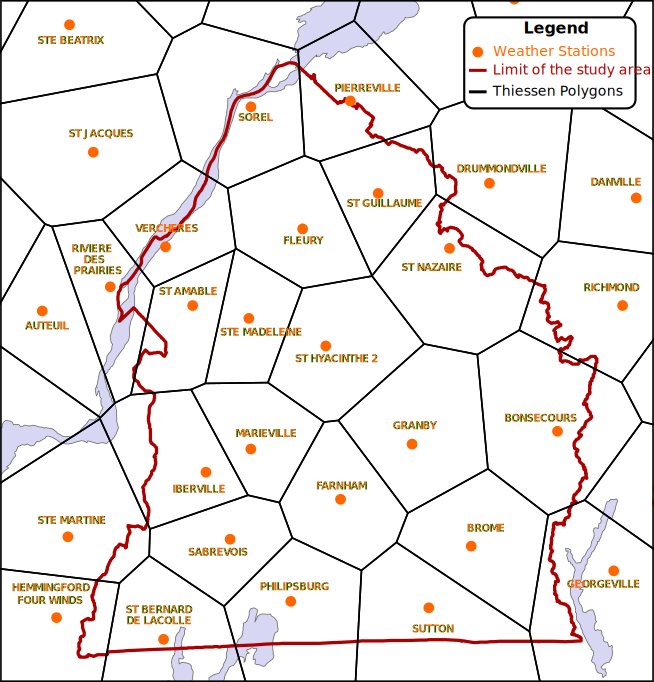
\includegraphics[width=0.75\textwidth]{img/Thiessen_meteo}
\caption[Locations of the weather stations in the Monteregie Est area.]{Locations of the weather stations in the Monteregie Est area.}
\label{fig:Thiessen_meteo}
\end{figure}


Tests have shown that inclusion of more than four stations does not significantly improve the interpolation and may in fact degrade the estimate. 

\subsection{Results and Discussion}

The quality of the estimates is strongly affected by seasonality. Stations at higher elevations are difficult to estimate accurately, in large part because of the topographical diversity of the surrounding stations leading to degradation of spatial coherence among stations.

The tendency for all of the methods to have a negative bias is indicative of the nature of precipitation distributions to be positively skewed (interpolated values will tend to cluster about the median error rather than the mean).

According to \cite{xia_forest_1999}, the two most important factors in climatology are the inter-correlations in the station network, and the seasonal variations in the relations between the stations.


\end{document}